\chapter{Definície a známe výsledky}
\label{chap:kapitola1}

Regulárny výraz (angl. \textit{regular expression}) je postupnosť znakov a metaznakov, ktorý definuje množinu reťazcov -- jazyk. Znaky zastupujú samé seba -- jednopísmenkový jazyk. Metaznaky majú symbolický význam -- popisujú, čo sa so znakmi/jazykmi pred alebo za nimi v postupnosti deje. Býva to konkrétny algoritmus, preto ich nazývame aj operácie. Začínajúc jednopísmenkovými jazykmi, pridávaním znakov, metaznakov a už vystavaných jazykov vieme poskladať zložitejšie jazyky.

Či slovo patrí do takto popísaného jazyka zistíme tak, že si súčasne prezeráme re\-gu\-lár\-ny výraz a slovo zľava doprava, pričom ak narazíme na operáciu, vykonáme ju. Chceme, aby sa slovo a regulárny výraz zhodovali v znakoch. Ak v oboch prídeme na koniec, slovo do jazyka patrí. Môže sa stať, že pri prezeraní budeme mať na výber, ako danú operáciu použiť, teda bude viacero 'rôznych prezeraní'. Nám postačí, ak takéto 'prezeranie', kde skončí slovo zároveň s regulárnym výrazom, existuje. Formálne ho\-vo\-rí\-me, že ak určité slovo patrí do popísaného jazyka, regulárny výraz \textbf{matchuje}\footnote{Bohužiaľ, slovenský ekvivalent tohto slova nie je taký výstižný, preto zostaneme pri anglickej verzii.} dané slovo, resp. zhoduje sa s ním alebo slovo pasuje.

Tieto postupnosti slúžia na vyhľadávanie slov\footnote{Lepšie by sa hodilo reťazcov, pretože myslíme ľubovoľný reťazec znakov definovaný nejakým re\-gu\-lár\-nym výrazom. Slovo v texte však väčšinou evokuje reťazec písmen s konkrétnym významom, slovo z jazykovedného hľadiska, čo momentálne nie je to, čo chceme.} v rôznych textoch pre ich ďalšie spracovanie ako napríklad prepísanie, vyznačenie pozície alebo informovaní o ich počte.

Keďže implementované regulárne výrazy sa už natoľko líšia od počiatočného teo\-re\-tic\-ké\-ho modelu -- nielen syntaxou ale aj triedou jazykov, ktorú popisujú -- zaužíval sa pre ne názov \textbf{regexy}. Budeme ho používať aj my a prípadnými predponami budeme rozlišovať, ktorú množinu operácií práve myslíme.

\section[Zákl. definícia]{Základná definícia regulárnych výrazov}
\label{def}

Samotný pojem \textbf{regex} bude slúžiť na pomenovanie regulárnych výrazov, ktoré pokrývajú triedu regulárnych jazykov. Z tohto dôvodu nebudeme vytvárať zvlášť pomenovanie pre túto triedu, bolo by to zbytočné. Pre ozrejmenie uvedieme základnú definíciu regexu z článku \cite{ExtendedRegexPower}. Niektoré konštrukcie sú oproti teoretickému modelu nové, ale dôkaz toho, že pokrýva stále rovnakú triedu jazykov, je triviálny.

\underline{Základná forma regexov}
\begin{list}{}{}
\item[(1)] Pre každé $a \in \Sigma$, $a$ je regex a $L(a)=\lbrace a \rbrace$. Poznamenajme, že pre každé $x \in \lbrace (,), \{, \},[,],\mathdollar,|, \backslash, .,?,*,+ \rbrace, \backslash x \in \Sigma $ a je regexom a $L(\backslash x) = \lbrace x \rbrace$. Naviac aj $\backslash n$ a $\backslash t$ patria do $\Sigma$ a oba sú regexami. $L(\backslash n)$ a $L(\backslash t)$ popisujú jazyky skladajúce sa z nového riadku a tabulátora.
\item[(2)] Pre regexy $e_1$ a $e_2$ 
\begin{list}{}{}
\item $(e_1)(e_2)$ (zreťazenie), 
\item $(e_1)|(e_2)$ (alternácia), a 
\item $(e_1)*$ (Kleeneho uzáver) 
\end{list}
sú regexy, kde $L((e_1)(e_2)) = L(e_1)L(e_2), L((e_1)|(e_2))=L(e_1) \cup L(e_2)$ a $L((e_1)*) = (L(e_1))^*$. Okrúhle zátvorky môžu byť vynechané. Ak sú vynechané, alternácia, zreťazenie a Kleeneho uzáver majú vyššiu prioritu.
\item[(3)] Regex je tvorený konečným počtom prvkov z (1) a (2).
\end{list}

\underline{Skrátnená forma}
\begin{list}{}{}
\item[(1)] Pre každý regex $e$: $(e)+$ je regex a $(e)+ \equiv e(e)*$.
\item[(2)] Znak ' . ' znamená ľubovolný znak okrem $\backslash n$.
\end{list}

\underline{Triedy znakov}
\begin{list}{}{}
\item[(1)] Pre $a_{i_1},a_{i_2},\dots ,a_{i_t} \in \Sigma,~t \geq 1,~\left[ a_{i_1}a_{i_2}\dots a_{i_t} \right] \equiv a_{i_1}|a_{i_2}|\dots |a_{i_t} $.
\item[(2)] Pre $a_i,a_j \in \Sigma$ také, že $a_i\leq a_j,~ [a_i-a_j]$ je regex a $[a_i-a_j]\equiv a_i|a_{i+1}|\dots |a_j$.
\item[(3)] Pre $a_{i_1},a_{i_2},\dots ,a_{i_t} \in \Sigma,~t \geq 1,~\left[ \textasciicircum a_{i_1}a_{i_2}\dots a_{i_t} \right] \equiv b_{i_1}|b_{i_2}|\dots |b_{i_s} $, kde $\lbrace b_{i_1}|b_{i_2}|\dots |b_{i_s}\rbrace = \Sigma - \lbrace a_{i_1},a_{i_2},\dots ,a_{i_t} \rbrace$.
\item[(4)] Pre $a_i,a_j \in \Sigma$ také, že $a_i\leq a_j,~ [a_i-a_j]$ je regex a $[\textasciicircum a_i-a_j]\equiv b_{i_1}|b_{i_2}|\dots |b_{i_s}$, kde $\lbrace b_{i_1}|b_{i_2}|\dots |b_{i_s}\rbrace = \Sigma - \lbrace a_i|a_{i+1}|\dots |a_j \rbrace$.
\item[(5)] Zmes (1) a (2) alebo (3) a (4).
\end{list}

\underline{Ukotvenie}
\begin{list}{}{}
\item[(1)] Znak pre začiatok riadku $ \textasciicircum $.
\item[(2)] Znak pre koniec riadku $ \mathdollar $.
\end{list}

Vo formálnom texte bude prirodzené pomenovávať ľubovoľný model regexov pomocou písmen gréckej abecedy.

Radi by sme spomenuli aj iné konštrukcie, ktoré v definícii chýbajú. V konečnom dôsledku síce modelu silu nepridajú, ale budeme s nimi počítať v ďalšom výskume, nakoľko sa bavíme o moderných regulárnych výrazoch.

\begin{list}{$\bullet$}{Nech $e$ je regex, potom}
\item $e*,e+?,e??$ je definované ako $e*,e+,e?$, ale snažia sa matchovať čo najmenej znakov ($*,+,?$ sú greedy)
\item $e\lbrace m \rbrace \equiv \underbrace{ee\ldots e}_m$ -- $m \in \N$ je konštanta; matchuje práve $m$ kópií daného regexu
\item $e \lbrace m,n \rbrace \equiv \underbrace{ee\ldots e}_n | \underbrace{ee\ldots e}_{n-1} | \dots | \underbrace{ee\ldots e}_m$ --  $m, n \in \N$ sú konštanty; matchuje aspoň $m$ a najviac $n$ kópií predošlého regexu, matchuje čo najviac
\item $e \lbrace m,n \rbrace ? \equiv \underbrace{ee\ldots e}_m | \underbrace{ee\ldots e}_{m+1} | \dots | \underbrace{ee\ldots e}_n$ -- čiže ako $ \lbrace m,n \rbrace$, ale snaží sa matchovať čo najmenej
\item $e(?\#\dots ) \equiv e$ -- komentár, pri matchovaní sa obsah ignoruje
\end{list}

Pre ľahší dôkaz uvedieme formálnu definíciu pre prvú operáciu a operáciu, ktorej algoritmus sa používa na simulovanie Kleeneho $*$.

\begin{df}[Minimalistická iterácia]
$$ L_{1} *? L_{2} = \lbrace uv ~|~ u \in L_1^* \land v \in L_2 \land u~je~najkratšie~také \rbrace $$
\end{df}

\begin{df}[Greedy iterácia]
$$ L_{1} \circledast L_{2} = \lbrace uv ~|~ u \in L_1^* \land v \in L_2 \land u~je~najdlhšie~také \rbrace$$
\end{df}

V sekcii \ref{iteracia} dokážeme, že tieto iterácie pokrývajú rovnakú triedu jazykov ako Kleeneho uzáver. Vidíme, že ostatné operácie sa ľahko prepíšu na už definované regexy, preto triedu jazykov nad regexami nerozšíria o žiaden nový jazyk. Poďme sa teda venovať tým zložitejsím a zaujímavejším operáciám.

\section{Spätné referencie}\label{chap:backref1}

Spätná referencia (angl. \textit{backreference}) je označovaná ako $ \backslash m $, kde $m \in \N$ je kon\-štan\-ta, a predstavuje reťazec, ktorý bol matchovaný obsahom $m$--tých okrúhlych zátvoriek. Okrúhle zátvorky číslujeme zľava doprava podľa poradia ľavej zátvorky. Samozrejme, $\backslash m$ môže ukazovať na zátvorky, ktoré obsahujú regex s inými spätnými referenciami. Vždy však budeme predpokladať, že spätná referencia s číslom $m$ sa bude nachádzať až za pravou zátvorkou s číslom $m$.

Poznamenajme, že ak sa $m$--té zátvorky nachádzajú vnútri Kleeneho $*$ a $\backslash m$ nie je vnútri tejto Kleeneho $*$, potom $\backslash m$ bude matchovať slovo z poslednej iterácie. Zároveň ak táto Kleeneho $*$ matchuje s nula iteráciami (t.j. $m$--té zátvorky sa k matchovaniu ani nedostanú), $\backslash m$ bude prázdny reťazec. To platí pre všetky prípady, kedy $m$--té zátvorky nič nematchujú.

Regexy rozšírené o spätné referencie (t.j. do abecedy regexov pribudne $\backslash m$, kde $m \in \N$) budeme nazývať \textbf{e-regex}. Triedu jazykov nad e-regexami budeme nazývať \textbf{Eregex}\footnote{Autori ju pôvodne nazvali extended regex resp. EREG, avšak pre lepšiu prehľadnosť v tejto práci sme názov upravili.}, presná definícia sa pochádza z článku \cite{ExtendedRegexPower}.  Narába s regexami uvedenými iba v úvodnej definícii, ale myslíme, že je zrejmé, že nové operácie nepridajú modelu silu, preto môžeme pracovať s touto rozšírenou množinou.

Označíme množinu podvýrazov vyskytujúcich sa v e-regexe $\alpha$ ako $SUB(\alpha )$. Rôzne výskyty identických podvýrazov sú považované za rôzne prvky $SUB(\alpha )$.

\begin{df}
\underline{Zhoda} (angl. match) e-regexu $\alpha$ je konečný (orientovaný, us\-po\-ria\-da\-ný) strom $T_\alpha$. Vrcholy $T_\alpha$ sú usporiadané podľa prvkov zo $\Sigma^* \times SUB(\alpha)$ a $T_\alpha$ je skonštruovaný podľa nasledujúcich pravidiel.
\begin{list}{}{}
\item[(i)] Koreň $T_\alpha$ je označený $(w,\alpha )$, $w \in \Sigma^*$.
\item[(ii)] Predpokladajme, že vrchol $u$ stromu $T_\alpha$ je označený ako $(w,\beta )$, kde $\beta = (\beta_1)(\beta_2) \in SUB(\alpha)$. Potom $u$ má dvoch synov, ktorí sú označený ako $(w_i,\beta_i),~i=1,2$ (v poradí), kde $w_1,w_2 \in \Sigma^*$ a platí $w = w_1w_2$.
\item[(iii)] Predpokladajme, že vrchol $u$ stromu $T_\alpha$ je označený ako $(w,\beta )$, kde $\beta = (\beta_1)|(\beta_2) \in SUB(\alpha)$. Potom $u$ má jedného syna, ktorý je jeden z prvkov $(w_i,\beta_i), ~ i \in \lbrace 1,2 \rbrace$.
\item[(iv)] Predpokladajme, že vrchol $u$ stromu $T_\alpha$ je označený ako $(w,\beta )$, kde $\beta = (\beta_1)* \in SUB(\alpha)$. Potom môžu nastať dva prípady: $w \neq \varepsilon$ alebo $w = \varepsilon$. Ak $w \neq \varepsilon$, $u$ má $k \geq 1$ synov označených ako
$$ (w_1,\beta_1), \ldots, (w_k,\beta_1) $$
kde $w_1 \cdots w_k = w, ~ w_i \neq \varepsilon, ~ i=1, \ldots ,k$. Ak $w = \varepsilon$, $u$ má jedného syna $u_1$ označeného $(\varepsilon , \beta )$ a $u_1$ je list $T_\alpha$.
\item[(v)] Ak sa $(w,a), ~ a\in \Sigma$ vyskytuje ako označenie nejakého vrchola $u$, potom nutne $u$ je list a $w=a$.
\item[(vi)] Ak sa $(w,\backslash m)$ vyskytuje ako označenie nejakého vrchola $u$, potom $u$ je list a $w \in \Sigma^*$ je určené nasledovne. Nech $\beta_m$ je podvýraz $\alpha$ uzavretý $m$--tým párom okrúhlych zátvoriek a nech $u_{\beta_m}$ je taký predchádzajúci vrchol $T_\alpha$ v štandardnom usporiadaní zľava-doprava, ktorý je označený prvkom, kde druhý komponent je $\beta_m $. Tento vrchol predchádza $u$ v uspriadaní vrcholov zľava-doprava. (Poznamenajme, že všetky vrcholy, ktorých označenie obsahuje $\beta_m$ sú nutne nezávislé, keďže sú lineárne usporiadané zľava doprava.) Potom zvolíme $w$ ako prvý komponent označenia $u_{\beta_m}$. Nakoniec, ak sa $\beta_m$ nevyskytuje v žiadnom označení vrchola $T_\alpha$, tak zadáme $w = \varepsilon$.
\end{list}
\end{df}

\begin{df}
\underline{Jazyk} rozpoznávaný e-regexom $\alpha$ je definovaný ako
$$ L(\alpha) = \lbrace w \in \Sigma^* ~|~(w,\alpha ) ~označuje~koreň~nejakej~zhody~T_\alpha \rbrace $$.
\end{df}

Dospelo sa k nasledujúcim výsledkom:
\begin{itemize}
\item V rámci Chomského hierarchie je trieda Eregex vlastnou podmnožinou $\L_{CS}$. Existujú jazyky z $\L_{CF}$ aj $\L_{CS}$, ktoré do nej nepatria.
\item Čo sa týka uzáverových vlastností, trieda je uzavretá na homomorfizmus a nie je uzavretá na komplement, inverzný homomorfizmus, konečnú substitúciu, shuffle s regulárnym jazykom. Neuzavretosť na prienik sa podarilo dokázať až v článku \cite{ExtendedRegexIntersec}.
\item Nekonečné jazyky z Eregex sa dajú pumpovať, dokázali sa už 2 verzie pumpovacej lemy (\cite[Lemma 1]{ExtendedRegexPower}, \cite[Lemma 3]{ExtendedRegexIntersec}).
\end{itemize}

\section{Lookaround}
\label{dflookaround}

Lookaround je spoločný názov pre dve operácie -- lookahead a lookbehind. Tieto operácie nás v práci budú zaujímať. Je to niečo nové a málo skúmané. Teraz si uvedieme ich popis a definície. Ako fungujú? 

Zoberme si lookahead. Už názov naznačuje, že to bude nazeranie dopredu. Myšlienka spočíva v tom, že si chceme povedať, čo má za nejakým hľadaným slovom nasledovať. Teda nájdeme slovo a potom nazrieme dopredu a overíme, či je tam práve to, čo chceme. Táto operácia 'nevyjedá' písmenká, čiže keď lookahead skončí a uspeje, pokračuje sa v ďalšom matchovaní akokeby tam nebol -- presne od toho miesta v slove, kde on začal pracovať. Presnejšie: slovo sa matchuje podľa regexu. Keď narazíme na look\-ahead, zapamätáme si toto miesto. Matchujeme podľa lookaheadu. Ak uspeje, potom sa v slove vrátime na zapamätané miesto a pokračujeme v matchovaní regexom za lookaheadom \cite{Python3Documentation}.

Lookbehind pracuje analogicky, ale pozerá sa dozadu -- teda chceme vedieť, čo hľadanému slovu predchádza. 

\begin{df}[Pozitívny lookahead]
$$ L_{1}(?=L_{2})L_{3} = \lbrace uvw ~|~ u \in L_{1} \land v \in L_{2} \land vw \in L_{3} \rbrace $$ Operáciu $(?=\dots)$ nazývame pozitívny lookahead alebo len \underline{lookahead}.
\end{df}

\begin{df}[Pozitívny lookbehind]
$$ L_{1}(?<=L_{2})L_{3} = \lbrace uvw ~|~ uv \in L_{1} \land v \in L_{2} \land w \in L_{3} \rbrace $$ Operáciu $(?<=\dots)$ nazývame pozitívny lookbehind alebo len \underline{lookbehind}.
\end{df}

Negatívna verzia funguje rovnako, ale otáča akceptačnú požiadavku -- namiesto toho, aby sme písali, čo nasleduje, definujeme práve to, čo nechceme aby nasledovalo. Teda negatívny lookaround 'zbehne', ak nie je schopný matchovať vstup.

\begin{df}[Negatívny lookahead]
$$ L_{1}(?!L_{2})L_{3} = \lbrace uv ~|~ u \in L_{1} \land v \in L_{3} \land neexistuje~také~x,y,~že~v=xy~a~x \in L_2 \rbrace $$ Operáciu $(?!\dots)$ nazývame \underline{negatívny lookahead}.
\end{df}

\begin{df}[Negatívny lookbehind]
$$ L_{1}(?<!L_{2})L_{3} = \lbrace uv ~|~ u \in L_{1} \land v \in L_{3} \land neexituje~také~x,y,~že~u=xy~a~y \in L_2 \rbrace $$ Operáciu $(?<!\dots)$ nazývame \underline{negatívny lookbehind}.
\end{df}

Ešte si definujme názvoslovie, aby sme vedeli pomenovať triedy a operácie, o ktorých budeme hovoriť.

\begin{df}
Množinu e-regexov rozšírenú o pozitívny lookahead a pozitívny lookbehind budeme nazývať \underline{le-regex}, triedu nad le-regexami \underline{LEregex}.
\end{df}

\begin{df}
Množinu le-regexov rozšírenú o negatívny lookahead a negatívny lookbehind budeme nazývať \underline{nle-regex}, triedu nad nle-regexami \underline{nLEregex}.
\end{df}

\section[Prax]{Regulárne výrazy v praxi}
\label{prax}

Už na začiatku sme spomínali, že táto práca je inšpirovaná novými konštrukciami, ktoré v praxi pribudli do modelu regulárnych výrazov. Pracovať s praktickým modelom však nie je také jednoduché. Pôvodná teoretická myšlienka narazí na prekážky implementácie a programátor sa musí rozhodnúť medzi tým, či ju splní do bodky alebo si ju niekde zjednoduší a zaručí tým rýchlejší algoritmus. V tejto podkapitole spomenieme obmedzenia, ktoré sú naimplementované a užívatelia regulárnych výrazov sa s nimi musia vysporiadať.

\begin{figure}[h]
  \centering
  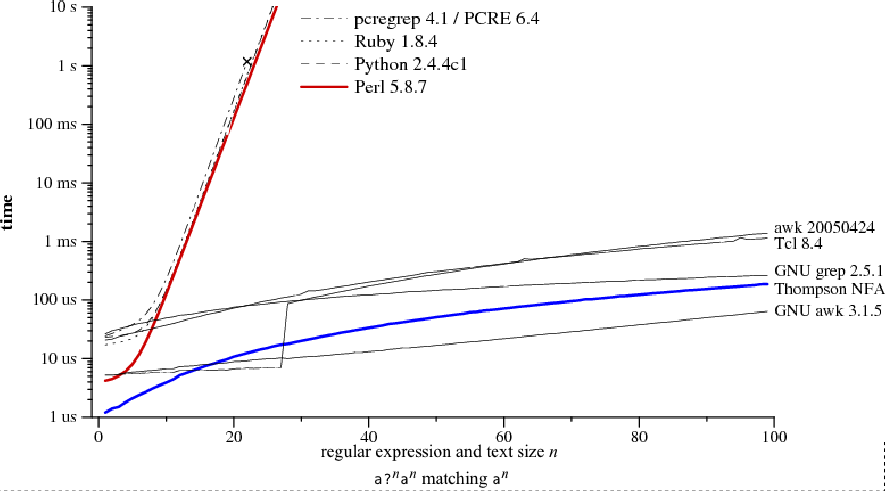
\includegraphics[width=1\textwidth]{obrazky/graf}
  \caption{Graf ukazuje čas potrebný na skontrolovanie, či $a^n?a^n$ matchuje $a^n$}
  \label{fig:graf}
\end{figure}
Za zmienku stojí fakt, že síce prvé implementácie používajú prevod na NKA a tak fungujú v lineárnom čase vzhľadom na veľkosť vstupu, ale v osemdesiatych rokoch tieto algoritmy ušli pozornosti Hernyho Spencera pri reimplementovaní a zverejnení ôsmej verzie Unixu, kam pre regulárne výrazy napísal algoritmus s exponenciálnou časovou zložitosťou využívajúci backtraking. Práve ten sa dostal do programovacích jazykov ako Perl, PCRE, Python, PHP, Ruby atď. Z neznámych dôvodov je tam dodnes a trápi užívateľov na kritických vstupoch (napr. match $a^n?a^n$ pre $n \geq 29$ trvá viac ako 10 sekúnd, viď Obr. \ref{fig:graf}), pričom, hoci už existujú spätné referencie a skutočne vyžadujú backtracking, by stačilo skontrolovať použitú syntax a podľa toho zvoliť algoritmus. Na druhej strane rýchly algoritmus sa nestratil úplne -- Unix a jeho aplikácie ho znova využívajú.

\subsection*{Regexy pokrývajúce triedu regulárnych jazykov}
\label{praxregex}

Trieda regulárnych jazykov je popísaná aj modelom konečných automatov. Tie sú ľahko implementovateľné, preto sa regexy simulujú pomocou nich. Ukážme si, ako funguje prevod medzi týmito dvoma modelmi.

\subsubsection{Thompsonov prevod regexu na nedeterministický konečný automat \cite{Cox07SlowPython}}

Máme regex $\alpha$ vystavaný z množiny operácií. My definujeme čiastočné NKA s voľnými šípkami pre jednotlivé operácie a tie sa potom podľa stavby $\alpha$ spoja do NKA pre $L(\alpha )$. Nakoniec voľné šípky z posledných operácií pripojíme na akceptačný stav. Ukážme si jednotlivé konštrukcie pre operácie, $e$ vždy bude označovať regex, ktorý nás zaujíma.
\begin{itemize}
\item $e=a,~a\in \Sigma$ -- matchovanie obyčajného znaku (t.j. nie metaznaku)
\begin{center}
	 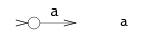
\includegraphics[scale=1]{obrazky/T_pismenko}
\end{center}
\item $e = e_1e_2$ zreťazenie -- koniec $e_1$ je pripojený na začiatok $e_2$
\begin{center}
    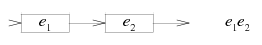
\includegraphics[scale=1]{obrazky/T_zretazenie}
\end{center} 
\item $e=e_1|e_2$ alternácia -- zo stavu sa nedeterministicky rozhodneme ísť buď vetvou $e_1$ alebo $e_2$
\begin{center}
    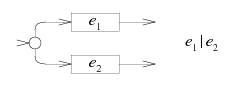
\includegraphics[scale = 1]{obrazky/T_alternacia}
\end{center}
\item $e*$ iterácia -- na $e$ je urobený cyklus. Nedeterministicky sa rozhodneme, koľkokrát ho absolvujeme. Samozrejme, môžeme iterovať aj nulakrát.
\begin{center}
    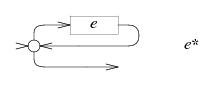
\includegraphics[width=0.40\textwidth]{obrazky/T_iteracia}
\end{center}
\item $e+$ plus -- opäť cyklus na $e$, ale samotné $e$ musí matchovať aspoň jedenkrát
\begin{center}
    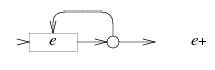
\includegraphics[scale=1]{obrazky/T_plus}
\end{center}
\item $e?$ otáznik -- nedeterministicky sa rozhodujeme, či ísť vetvou $e$ alebo $\varepsilon$
\begin{center}
    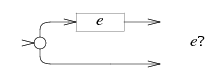
\includegraphics[scale=1]{obrazky/T_otaznik}
\end{center}
\item zvyšok syntaxe je možné prepísať pomocou predošlých znakov a metaznakov
\end{itemize}

Každý znak a metaznak (okrem okrúhlych zátvoriek) pridáva NKA jeden stav, teda počet stavov je najviac rovný dĺžke prevádzaného regexu.

Vidíme, že v praxi v tejto oblasti problém nie je. Opísané prevedenie na nedeterministický konečný automat je rýchle -- stačí jeden prechod celého regexu. Potom niektoré implementácie pokračujú prevodom na deterministický automat, prípadne urobia úpravy na niečo medzi (napr. odepsilonovanie). Nás\-led\-ná simulácia konečného automatu má lineárnu časovú zložitosť vzhľadom na dĺžku prehľadávaného textu\cite{ExtendedRegexPower}. Nanešťastie nie všetky prostredia s regulárnymi výrazmi využívajú tento algorimus. No aj keď pracujú s backtrackingom, neokliešťujú regulárne výrazy o žiadnu funkcionalitu. Jedinou zmenou je prevedenie Kleeneho $*$ (teda aj $+$ a $?$), kedy sa používa greedy verzia -- snaží sa matchovať čo najdlší reťazec, ale ako sme spomenuli v \ref{def}, nevadí to.

\subsection*{Spätné referencie}
\label{praxbackref}

Majú v praxi povolené najviac trojciferné čísla\cite{Python3Documentation}, aby bolo ľahšie rozlíšiteľné, čo ešte referencia je a čo už nie, a celkovo z hľadiska časovej a pamäťovej zložitosti algoritmu. Na druhej strane teoretický model sa takýmito problémami nemusí zaoberať, preto povolíme všetky možné konštanty.

\subsection*{Lookaround}
\label{praxla}

Ako prvé si všimnime významný rozdiel medzi definíciou a reálnym modelom. Re\-gu\-lár\-ne výrazy sa začali využívať na vyhľadávanie v texte a v tomto kontexte má lookaround iný význam ako v teoretickom prostredí. Využíva sa to, že nevyjedá písmenká a preto sa dá použiť v takých prípadoch, kedy si chceme označiť slovo $w$, ale vieme, že hľadáme slovo $v$, pričom $w$ je podslovo $v$. Teda v takom prípade môže look\-ahead ďaleko presahovať slovo, na ktoré sme vyhlásili zhodu. Z toho vyplýva, že my by sme na vstup nechceli dostať $w$, ale $v$. V teoretickom prostredí nás však zaujíma slovo, ktoré do jazyka patrí a na jeho okolie sa nepozeráme, v podstate ho ani nemáme k dispozícii. Preto sa zdá, že budeme na vstupe očakávať $w$ a lookahead či lookbehind nebudú môcť presahovať za hranice slova. Táto úprava však neuškodí, nakoľko vieme z daného $w$ spraviť $v$ jednoduchým pridaním $(.*)$ na správne miesta.

Ďalšou črtou praktického prevedenia je, že programátori si definovali lookahead a lookbehind ako \textbf{atomické operácie}\cite{LApracticalnote}. To znamená, že matchovanie regexu vnútri lookaroundu prebieha normálne, ale akonáhle splní matchujúcu podmienku, celý výpočet aj s medzivýsledkami upadne do zabudnutia a žiaden back\-tracking zvonku už nebude schopný meniť ich vnútorný výpočet. Na prvý pohľad sa zdá, že to nemôže až tak prekážať, no opak je pravdou. Predstavme si lookaround, ktorý obsahuje okrúhle zátvorky, na ktoré sa odvolávajú spätné referencie niekde vonku ďalej v regexe. Z čoho vyplýva, že iné matchovanie v lookarounde (s rovnakým výsledkom) by mohlo ovplyvniť matchovanie regexu ako celku.

Napríklad le-regex $(?=([0-9]+))[+-*/]\backslash 1$ by mal matchovať reťazce typu číslo--operácia--číslo, ale my vieme, že nebude matchovať slovo $123+12$. Vyplýva to z toho, že $+$ je greedy a lookahead je atomický. S backtrackingom by toto nenastalo.

\subsubsection{Lookbehind}
\label{praxlb}

Simulácia lookaheadu je jednoduchá -- vieme, kde začína, teda ho spustíme od tohto miesta a čakáme na výsledok. Taký lookbehind sa však pozerá dozadu, teda potrebujeme určiť, kde začať. V praxi by sa toto riešilo backtrackingom, lebo nevieme vopred ako ďaleko dozadu sa budeme potrebovať pozrieť. Najprv by sme vyskúšali jeden znak a pri neúspechu by sme testovaný reťazec predlžovali. Backtracking je však drahý na čas a keďže autori programovacích jazykov nechceli príliš spomaľovať výpočty a asi nepovažovali lookbehind za taký dôležitý, určili si, že môže obsahovať iba také regexy, z ktorých je jasne určiteľné aký dlhý reťazec bude lookbehind potrebovať na výpočet ešte predtým ako sa spustí (takže sa backtrackingu vyhli)\cite{LApracticalnote}. 

\subsection*{Na záver}
\label{praxzaver}

Jedným dychom s týmito obmedzeniami dodávame, že my sa nachádzame v teo\-re\-tic\-kom prostredí, preto nás implementačné prekážky trápiť nemusia. Budeme pracovať s plným (čiže silnejším) modelom, aký je popísaný v definíciách. Z čoho je jasné, že ten reálny bude akousi jeho pod\-mno\-ži\-nou. Preto dokázané výsledky budú tvoriť hornú hranicu toho, čo sme v praxi schopní dokázať a keby niekto inovatívny implementoval operácie v ich plnej sile, tento model stále dobre poslúži.